\section{Overview}
\label{sec:overview}

\PurePy is a subset of Python chosen so that its programs are well-behaved and broadly \emph{pure}, yet run
unchanged under a standard Python interpreter and compute the same result. \secref{purity} makes the purity
claim precise and sets out the excluded features, grouped by the discipline each one protects;
\figref{prevented-errors} summarises the Python runtime errors that well-formedness rules out, and
\figref{roadmap} lists planned additions and features under consideration.

\subsection{Python compatibility}
\label{sec:python-compatibility}

\PurePy is a subset of Python: every well-formed program is a syntactically valid Python program, and if \PurePy
gives a run a result, that run produces the same result under Python. \paperonly{\figref{taxonomy} shows the
relationship between the two languages, with the guarantee appearing as containment.}

Well-formedness is a property of the program, decided by \PurePy's static checks. Semantic validity is
a property of a run rather than a program, because some of the Python behaviours \PurePy excludes cannot be rejected
statically (\secref{no-coercions}). An implementation may report a dynamically excluded operation by raising
\pyinline{UnsupportedOperationError}, but is not obliged to. The guarantee covers only valid runs, and a
stock Python interpreter will simply produce the Python result. \added{An implementation conforms if it accepts
exactly the well-formed programs and, on every valid run, produces the Python result.} The conformance suite is
organised the same way\paperonly{ (\secref{reference-impl})}\speconly{ (\secref{testing})}.


\begin{figure}
\centering
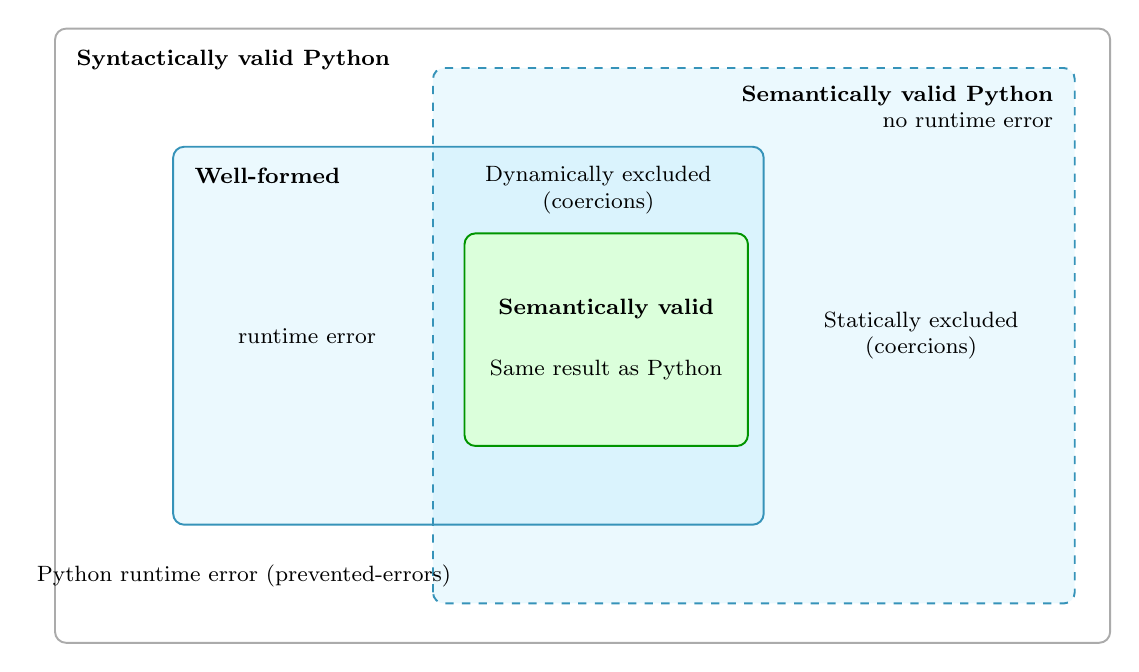
\begin{tikzpicture}[font=\footnotesize, rounded corners=4pt]
  \fill[cyan!60, fill opacity=0.13] (4.8,0.5) rectangle (12.95,7.3);
  \fill[cyan!60, fill opacity=0.13] (1.5,1.5) rectangle (9.0,6.3);
  \fill[green!14] (5.2,2.5) rectangle (8.8,5.2);
  \draw[black!33, line width=0.7pt] (0,0) rectangle (13.4,7.8);
  \draw[cyan!72!black, line width=0.7pt] (1.5,1.5) rectangle (9.0,6.3);
  \draw[dashed, cyan!72!black, line width=0.7pt] (4.8,0.5) rectangle (12.95,7.3);
  \draw[green!58!black, line width=0.7pt] (5.2,2.5) rectangle (8.8,5.2);
  \node[anchor=north west] at (0.15,7.65) {\textbf{Syntactically valid Python}};
  \node[anchor=north east, align=right] at (12.8,7.2) {\textbf{Semantically valid Python}\\no runtime error};
  \node[anchor=north west] at (1.65,6.15) {\textbf{Well-formed \PurePy}};
  \node[align=center] at (2.4,0.85) {Python runtime error (\figref{prevented-errors})};
  \node[align=center] at (11.0,3.9) {Statically excluded\\(\figref{coercions})};
  \node[align=center] at (3.2,3.9) {\PurePy runtime error};
  \node[align=center] at (6.9,5.75) {Dynamically excluded\\(\figref{coercions})};
  \node[align=center] at (7.0,3.85) {\textbf{Semantically valid}\\\textbf{\PurePy}\\[1mm]Same result as Python};
\end{tikzpicture}
\caption{Python programs and runs, classified by \PurePy}
\label{fig:taxonomy}
\end{figure}

\todo{Python has no variable declarations, so a name's binding structure is not evident from the syntax.
This motivates the definite-assignment analysis (\secref{well-formedness}).}

\subsection{Purity}
\label{sec:purity}

\PurePy is not semantically ``pure'' in the sense of providing a guarantee that every program terminates with
a unique value. No practical programming language is pure in this sense. Real programs may fail to terminate,
or abort with errors such as division-by-zero or index-out-of-bounds, even in languages regarded as (mostly)
pure, like Haskell.

We do, however, claim that \PurePy is pure in the senses that matter. Every name has a unique lexical scope; a
variable, once definitely assigned, denotes a fixed value; a module's members are fixed once the module has
loaded. There is no mutation, nor can evaluation order change the meaning of a name. Python operates largely
outside this discipline, and the goal of \PurePy is to characterise a suitably large subset of Python that
stays within it.

A non-trivial component of the PurePy specification concerns module loading, in the form of well-formedness
rules which rule out programs which depend on Python's load-order-sensitive behaviours
(\secref{no-load-dependent}). One might wonder why a language which is mutation-free even needs to concern
itself with loading order. If the result of a program is all that can be observed, the order in which
subexpressions are evaluated cannot affect that result, and so cannot meaningfully be part of the
specification. However runtime errors, at least if they can be distinguished, remove that freedom: if
division-by-zero reports differently from index-out-of-bounds, a program with two possible failures reveals
which was reached first, and implementations which choose different orders might disagree about what such a
program does. \PurePy aims to serve as a template for practical implementation, not as an idealised calculus,
and practical implementations need to be able to report on different kinds of error, since those reports are
important to users. The sequential semantics of module loading therefore remains an important part of the
specification so that programs which fail do so deterministically under every implementation.

Real-world languages, including the ``pure'' ones, also support logging to a terminal. Haskell has
\pyinline{trace}; \PurePy has \pyinline{print}, following Python. This too is a computational effect, but one
that is not only indispensable but benign; printing can only report on a computation and cannot influence its
result. Moreover with loading order already part of the specification, printing is a low-cost, high-utility
feature that leaves the core purity benefits of \PurePy untouched.

\subsubsection{Mutable state}
\label{sec:no-mutable-state}

A variable in \PurePy denotes a fixed value once definitely assigned, so features that mutate or rebind state
are excluded: \pyinline{global} and \pyinline{nonlocal}, which reassign bindings in an outer scope;
\pyinline{del}, which removes a binding; augmented assignment (\pyinline{+=}, \pyinline{-=}, and so on); and
the walrus operator (\pyinline{:=}), which assigns within an expression. Reassignment of a variable already
captured by a closure is excluded for the same reason. In Python a closure captures a mutable binding, so a
later reassignment is visible through the closure:

\begin{python}
def f():
    x = 5
    def g():
        return x
    x = 6
    return x + g()
\end{python}

\noindent Here \pyinline{g()} returns \pyinline{6} in Python and the result is \pyinline{12}; under a pure
reading in which \pyinline{x = 6} shadows the earlier binding, \pyinline{g()} would return \pyinline{5} and the
result \pyinline{11}. \PurePy rejects the program, keeping closures over values rather than mutable cells, as
with Java's requirement that captured locals be effectively final~\cite[\S15.27.2]{gosling2025}. The rules that
enforce this are given in \secref{captured-vars}.

\subsubsection{Control flow and effects}
\label{sec:no-effects}

\PurePy excludes loops with \pyinline{break} and \pyinline{continue}, exceptions
(\pyinline{try}/\allowbreak\pyinline{except}/\allowbreak\pyinline{raise}), context managers (\pyinline{with}), generators
(\pyinline{yield}/\allowbreak\pyinline{yield from}), and coroutines (\pyinline{async}/\allowbreak\pyinline{await}). Functional
programming has rich accounts of effects, from monads to algebraic effect handlers, so these features are not
inherently at odds with a functional language. In idiomatic Python, though, they are used mainly in
conjunction with mutable state, which \PurePy already excludes, and iteration is expressed by comprehensions
and recursion rather than by loops. A future release may add structured effects; for now the core stays
effect-free.

\subsubsection{Implicit coercions}
\label{sec:no-coercions}

Python accepts several implicit coercions and lax matches. \figref{coercions} lists those \PurePy
excludes, and records at which stage each exclusion takes effect. A dynamically excluded operation leaves
the run without a result, so the program runs under Python but not under \PurePy.

\begin{figure}
\centering
\small
\setlength{\tabcolsep}{4pt}
\begin{tabular}{>{\raggedright\arraybackslash}p{0.20\textwidth}>{\raggedright\arraybackslash}p{0.315\textwidth}>{\raggedright\arraybackslash}p{0.25\textwidth}>{\raggedright\arraybackslash}p{0.142\textwidth}}
\hline
\textbf{Construct} & \textbf{Python} & \textbf{\PurePy} & \textbf{Excluded} \\
\hline
Tests of \pyinline{if} and \pyinline{assert} & Coerced to \pyinline{bool} & Must already be Boolean & Dynamically \\[1mm]
Sequence patterns & List patterns match tuples, and tuple patterns lists & List patterns match only lists, tuple patterns only tuples & Dynamically \\[1mm]
Constructor patterns & Positional class patterns may supply fewer sub-patterns than the class has fields & Require exact arity & Statically \\[1mm]
Dictionary keys & Any hashable value, with \pyinline{1}, \pyinline{1.0} and \pyinline{True} equivalent as keys & Strings only & Statically in patterns, dynamically in expressions \\[1mm]
\pyinline{assert} message & Any object, shown in the traceback & Strings only & Dynamically \\[1mm]
\pyinline{==} and \pyinline{!=} & Compare any two operands, giving \pyinline{False} when unrelated & Undefined between, say, number and string, or list and tuple; only \pyinline{None} compares with anything & Dynamically \\[1mm]
Functions under \pyinline{==} & Compared by identity, so two textually identical lambdas are unequal & Equality undefined & Dynamically \\[1mm]
\pyinline{nan} comparison via container equality & Elements compared by identity before equality, so identical NaNs match but distinct ones do not & Undefined when both elements are \pyinline{nan} & Dynamically \\
\hline
\end{tabular}
\caption{Python coercions and lax matches excluded by \PurePy}
\label{fig:coercions}
\end{figure}



\subsubsection{Load-dependent meaning}
\label{sec:no-load-dependent}

A name's meaning in \PurePy must not depend on the order in which modules load or on runtime state, so several
of Python's import and module behaviours are excluded. Imports must appear at the start of a module, never
inside a function or other block, nor after a non-import statement. Wildcard imports (\pyinline{from q import
*}) are excluded, since the names they introduce are not explicit; PEP 8 recommends against
them.\footnote{\url{https://peps.python.org/pep-0008/}} A submodule may not import itself through its parent
(\pyinline{from a import b} inside module \pyinline{a.b}): \PurePy treats the from-imported submodule as a
dependency, so this is an import cycle. An \pyinline{import} (as opposed to a from-import) may not name a proper
descendant of the importing module (\pyinline{import x.y} inside module \pyinline{x}), since the binding for
the head would denote the still-loading module.

A module may not bind a name that is also the name of one of its submodules. In Python an attribute of a
package can be set both by an assignment in the package body and by loading the same-named submodule, and which
wins depends on load order. Consider a program with four modules:

\begin{minipage}[t]{0.2\textwidth}
\begin{python}
# pkg
sub = 1
\end{python}
\end{minipage}
\hfill
\begin{minipage}[t]{0.2\textwidth}
\begin{python}
# pkg.sub
# (empty)
\end{python}
\end{minipage}
\hfill
\begin{minipage}[t]{0.25\textwidth}
\begin{python}
# helper
import pkg.sub
\end{python}
\end{minipage}
\hfill
\begin{minipage}[t]{0.28\textwidth}
\begin{python}
# __main__
import pkg
print(pkg.sub)  # 1
\end{python}
\end{minipage}

Here \pyinline{helper} is never imported, so \pyinline{pkg.sub} never loads, and \pyinline{pkg.sub} in the
main module denotes the assignment. Now let the main module also import \pyinline{helper}, which it does not
otherwise use:

\begin{center}
\begin{minipage}[t]{0.55\textwidth}
\begin{python}
# __main__
import helper
import pkg
print(pkg.sub)  # <module 'pkg.sub'>
\end{python}
\end{minipage}
\end{center}

Loading \pyinline{pkg.sub}, wherever in the program it happens, sets it as an attribute of the shared
\pyinline{pkg} object, so the extra import changes what \pyinline{pkg.sub} means in a module that never
mentions \pyinline{pkg.sub}. The name has no load-order-independent meaning, so \PurePy excludes the clash
outright.

For the same reason, a module may not refer to a submodule it does not itself import. A submodule is not an
attribute of its package until it is loaded, so \pyinline{import a} followed by \pyinline{a.b.f()} is rejected
unless the module also imports \pyinline{a.b}; Python permits the reference whenever some earlier import,
anywhere in the program, happens to have loaded \pyinline{a.b}. \PurePy likewise rejects a reference to a
module member the module body never assigns, such as \pyinline{lib.x} where \pyinline{lib} assigns
\pyinline{x} only on a branch that is not taken. In Python both cases raise \pyinline{AttributeError}; \PurePy
rejects them statically.

\subsubsection{Modules and classes are not first-class}
\label{sec:no-first-class}

For now, modules and classes are not values in \PurePy. In Python a module is a value and a class declaration
is an assignment, so both flow through programs as data. Treating them as first-class would complicate the
static account, so the present subset keeps them second-class rather than ruling the feature out; a later
release may revisit it. A module name may be projected by member access but not used as a value, and a class
name appears only at constructor and pattern positions, with declarations confined to module level. Because a
class is identified by its qualified name, a dataclass declaration may not re-declare a name that already
denotes a class in the module; Python permits the re-declaration, leaving the earlier class reachable only
through its existing instances.

\subsubsection{Other restrictions}
\label{sec:other-restrictions}

A few remaining restrictions do not fit the groups above. A \pyinline{class} definition must be a
dataclass, and a dataclass body declares fields and nothing else. \PurePy therefore supports none of Python's
class-based extension mechanisms, such as \pyinline{__getitem__} for subscripting, \pyinline{__iter__} for
iteration or \pyinline{__eq__} for equality. Subscripting, iteration, equality and membership have the fixed
meanings given in \secref{opsem}.

\subsubsection{Runtime errors}
\label{sec:runtime-errors}

A well-formed \PurePy program avoids the Python runtime errors listed in
\figref{prevented-errors}, under the conditions noted there. Well-formedness does not prevent errors from
ill-typed operations, such as wrong operand types, calling a non-function, calling a function with the
wrong number of arguments, or attribute access on an object lacking the attribute. Each of these has a termination kind and a rule in the semantics\speconly{ (\figref{eval-fails})}.

\begin{figure}
\centering
\small
\begin{tabular}{>{\raggedright\arraybackslash}p{0.23\textwidth}>{\raggedright\arraybackslash}p{0.55\textwidth}>{\raggedright\arraybackslash}p{0.12\textwidth}}
\hline
\textbf{Python error} & \textbf{Ruled out when} & \textbf{See} \\
\hline
\pyinline{NameError}, \pyinline{UnboundLocalError} & Always: a variable may be referenced only where it is definitely assigned. & \figref{well-formed}, \figref{well-formed-expr} \\[1mm]
\pyinline{ModuleNotFoundError} & Always: an import requires its target to be a module of the program. & \figref{well-formed-imports} \\[1mm]
\pyinline{ImportError} & Always: a from-import requires each imported name to be a member of the source module, and import cycles are rejected. (A Python cycle may run or fail, depending on where the cycle is entered.) & \figref{imports}, \figref{well-formed-module} \\[1mm]
\pyinline{AttributeError} & The reference is a module attribute, which must resolve to a definitely assigned member.  & \figref{well-formed-expr} \\[1mm]
\pyinline{TypeError} & The operation is a constructor call or class pattern, which must match the class's arity exactly. (Only excess sub-patterns are a Python error; a pattern with fewer is excluded even though Python permits it.) & \figref{well-formed-expr}, \figref{well-formed-pat} \\
\hline
\end{tabular}
\caption{Python errors prevented by well-formedness}
\label{fig:prevented-errors}
\end{figure}



\begin{figure}
\small
\begin{center}
\begin{minipage}[t]{0.4\textwidth}
\vspace{0pt}
\begin{tabular}{ll}
\textbf{To do} & \\
Reserved words & \issue{9} \\
Set expressions & \issue{147} \\
Identity operator (\pyinline{is}) & \issue{81} \\
Chained comparison & \issue{82} \\
Enums & \issue{86} \\
Aliased imports & \issue{135} \\
Ints and floats & \issue{156} \\
\end{tabular}
\end{minipage}\hspace{2em}
\begin{minipage}[t]{0.4\textwidth}
\vspace{0pt}
\begin{tabular}{ll}
\textbf{Under consideration} & \\
Destructuring assignment & \issue{54} \\
f-strings & \issue{55} \\
Default arguments & \issue{56} \\
\pyinline{*args} and \pyinline{**kwargs} & \issue{57} \\
\deleted{Decorators} & \deleted{\issue{58}} \\
Slicing & \issue{59} \\
Star patterns & \issue{84} \\
Or patterns & \issue{85} \\
Relative imports & \issue{126} \\
Wildcard imports & \issue{105} \\
Function keyword arguments & \issue{127} \\
Postponed annotation evaluation & \issue{128} \\
Primitive operations & \issue{132} \\
\end{tabular}
\end{minipage}
\end{center}
\caption{\todo{Planned additions and features under consideration}}
\label{fig:roadmap}
\end{figure}

